\subsection{DETER}
\label{subsection:DETER}

Dans le domaine de la cyber-sécurité, le test de solutions de défenses proposées
face aux différentes menaces n'est pas simple et se développe lentement. En
effet, de nombreuses ressources sont nécessaires et il ne semble pas judicieux
d'effectuer les tests en environnement réel. De plus, les innovations qui
fonctionnent parfaitement dans des environnements contrôlés et prédictibles
sont souvent moins efficaces et fiables dans la réalité de par la taille du
réseau et des ressources qui constituent son environnement.  C'est pour cela que
l'USC\footnote{University Southern California} et l'UC
Berkeley\footnote{Université de Californie à Berkeley} ont lancé le projet DETER
\citep{DETER_Project, DETER_benzel2011science, DETER_mirkovic2010deter}. À sa
création en 2003, DETER était un projet de recherche avancée visant à
développer des méthodes expérimentales pour les innovations en matière de
cyber-sécurité (contrer les cyber-attaques, trouver les failles réseaux
...). Puis en 2004, le besoin de tester ces méthodes se faisant de plus en plus
sentir, le développement de DeterLab\footnote{DeterLab: cyber DEfense Technology
  Experimental Research Laboratory} a été lancé. Cette plateforme d'émulation
par interception libre et partagée fournit un environnement de test large
échelle et réaliste. Elle permet également d'automatiser et de reproduire des
expériences pouvant être de différentes natures. En effet, DeterLab peut
\textit{i)} observer et analyser le comportement de cyber-attaques\footnote{
  Attaques DDos et botnets, vers et codes malicieux, protocoles de stockage
  anti-intrusion (intrusion-tolerant), ainsi que le chiffrement et la détection
  de \textit{pattern}.} et de technologies de cyber-défense, \textit{ii)} tester et
mesurer l'efficacité des solutions de défenses proposées pour contrer les
menaces. Les utilisateurs accèdent aux machines dont ils ont besoin pour leurs
expériences, demandent une certaine configuration du réseau, du système et des
applications présente sur les machines. Pour fonctionner, ce laboratoire virtuel a
développé 7 outils complémentaires. Seuls 4 outils nous intéressent dans le cadre de notre projet\footnote{Les 3 autres sont le simulateur de comportement humain DASH, ``Multy-party Experiments'' pour avoir une vision partielle du monde lors d'une expérience et ``Risky Experiment Management Capability'' pour gérer les échanges d'expériences avec le réseau extérieur.}.

Le premier, qui constitue le c\oe ur logiciel et hardware de DeterLab, se base
sur Emulab \citep{EMULAB_INIT}. DeterLab a étendu ce dernier pour permettre de
faire des tests large échelle spécialisés dans le domaine de la cyber-sécurité
et dont la complexité est représentative des réseaux d'aujourd'hui (nombre de
n\oe uds, hétérogénéité des plateformes, contrôle de la bande passante et
délai). Il fournit également une interface web pour gérer à distance ses
expériences, les projets en développement et accéder aux autres outils de
DeterLab.

\begin{figure}
  \centering 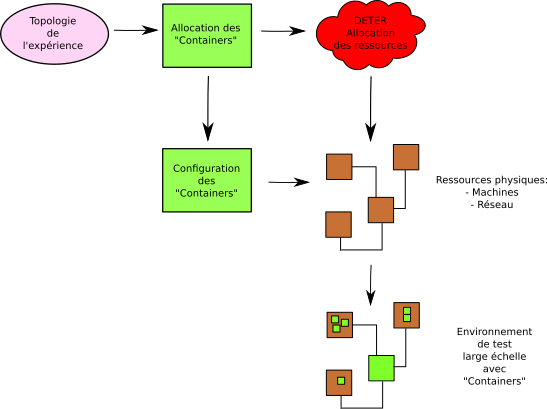
\includegraphics[scale=0.75]{Pictures/png/Deter_fonctionnement_container_v2}
  \caption{Diagramme du fonctionnement d'un \textit{Container}.}
  \label{Conteneur}
\end{figure}

Pour gérer les ressources nécessaires à leurs expériences, les
chercheurs du projet DETER ont créé ``The DeterLab Containers''
(Figure \ref{Conteneur}). Ces derniers permettent de virtualiser les
ressources et donc de répartir la puissance de calcul là où elle est
nécessaire. Ainsi, pour des ressources nécessitant une machine entière,
le conteneur sera la machine alors que pour une ressource qui n'aura
besoin que d'une partie de la machine, le conteneur sera une
abstraction de cette partie de la machine contenant les ressources
utilisées par l'application. Cela permet d'isoler les tests qui
n'utilisent pas une machine complète et de partager ses ressources
entre plusieurs tests concurrents. Ce mécanisme de virtualisation
s'appelle la ``Multi-resolution Virtualization''.

Actuellement, il existe plusieurs plateformes de tests basées sur Emulab avec
des extensions pour pouvoir être utilisées dans des domaines spécifiques comme
le fait DETER. Il se peut qu'une expérience exécutée sur une de ces plateformes
aie besoin de plus de machines que la plateforme ne peut en fournir, que ce soit
en terme de nombre, de puissance ou d'hétérogénéité des machines. Pour pallier
ce problème, le projet DETER a créé la
``Federation''\citep{DETER_faber2007deter}. Elle permet de déployer une
expérience sur plusieurs plateforme de tests différentes et d'avoir un plus
grand facteur de passage à l'échelle. La Figure \ref{Federation} montre
l'exécution d'une expérience dont les 3 n\oe uds sont répartis sur différentes
plateformes. La difficulté ici est que les plateformes sont contrôlées par des
propriétaires différents ayant des règles de sécurité d'accès souvent très
différentes de celles du projet DETER.

-\begin{figure}
  \centering 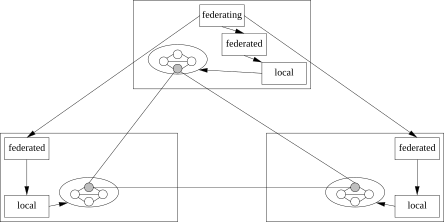
\includegraphics[scale=0.75]{Pictures/png/Deter_federation}
  \caption{Fédération d'une expérience répartie sur 3 plateformes de tests différentes.}
  \label{Federation}
\end{figure}

Pour que cette solution fonctionne, les plateformes vont partager un système de
nommage permettant de ne pas montrer à l'application la répartition de ses
ressources sur le réseau et une authentification pour contrôler l'accès d'une
plateforme à une autre. Pour gérer cela on va utiliser trois types de n\oe uds
différents (Figure \ref{Federation}). Le premier est le ``federating'', il est
unique et se place sur la plateforme qui demande à exécuter une expérience. Il
cherche les ressources disponibles sur les différentes plateforme puis divise
l'expérience en sous-expérience qu'il assigne à chaque plateforme. Il gère
l'exécution de l'expérience, récupère les données à la fin et
libère les ressources utilisées. Le second type de n\oe ud est le ``federated'',
on en place un sur chaque plateforme. C'est lui qui fournit la liste des
ressources disponibles sur sa plateforme de tests et qui configure les
sous-expériences qu'il reçoit du federating. Il fait la traduction de nom entre
le federating, qui utilise le système de nommage partagé, et le réseau local qui
utilise son système de nommage spécifique.  Il gère également la mise en place
des connexions réseaux entre les entités réparties sur les différentes
plateformes. Le dernier n\oe ud appelé ``local'' est également présent sur
chaque plateforme où l'expérience va s'exécuter. Il gère les communications
entre les différentes plateformes et les sécurise pour éviter les fuites à
l'extérieur du réseau ou l'espionnage par d'autres applications s'exécutant sur
la même plateforme.

Pour finir, MAGI\footnote{Montage AGent Infrastructure} fournit un système de
gestion de flux entre les différentes entités d'une expérience, permettant ainsi
d'avoir un certain contrôle sur les machines. En gérant le flux, on peut
automatiser et reproduire les expériences. En effet, MAGI capture chaque
séquence d'instructions concurrentes que l'expérience va suivre pour gérer le
flux, ainsi on peut rejouer la capture plus tard avec les paramètres d'origine
ou des nouveaux si un fichier de paramètres à tester existe. MAGI permet
également de visualiser l'évolution d'une expérience en cours d'exécution pour
s'assurer que son comportement reste correct sans avoir à attendre le résultat
final. En capturant les configurations demandées par les utilisateurs, MAGI
permet leur réutilisation par d'autres utilisateurs pour éviter à DETER de
reconstruire la même architecture pour une prochaine expérience.

\begin{figure}[H]
\centering
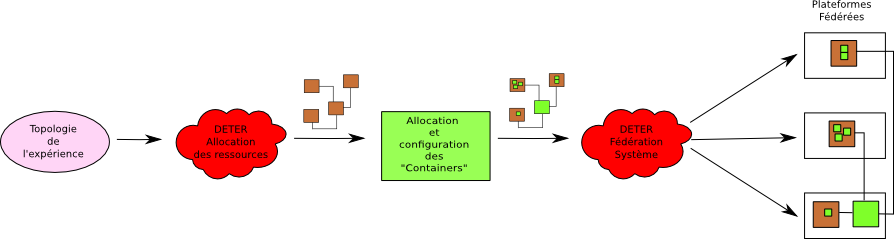
\includegraphics[scale=0.63]{Pictures/png/Deter_fonctionnement_general}
\caption{Création de l'environnement d'une expérience.}
\label{Deter_fonc}
\end{figure}

 Actuellement, DeterLab peut émuler des dizaines de milliers de n\oe uds: le
 projet dispose de 500 machines et 10 FPGA. Il est le seul émulateur dans le
 domaine de la cyber-sécurité et permet de faire des tests large échelle dont la
 complexité est représentative des réseaux.
